\newpage
\section*{二、实验操作与原始数据}


\subsection*{1. 实验条件与原始记录}

本次使用 FB807 型光电效应测定仪。截止电压及伏安特性测量均采用 4 mm 光阑，光源距离为 400 mm；五片滤光片波长分别为 365、405、436、546、577 nm。截止电压实际各测三次，共15个读数；伏安特性每个波长记录23个电压点，共115个数据点。

采用零电流法，在小电流档调节反向电压，记录电流为零时的带符号电压。伏安特性使用较大电流档逐点记录；拓展实验在365 nm、20.00 V条件下分别改变距离和孔径，下图为调试过程现场图片。

\begin{figure}[H]\centering
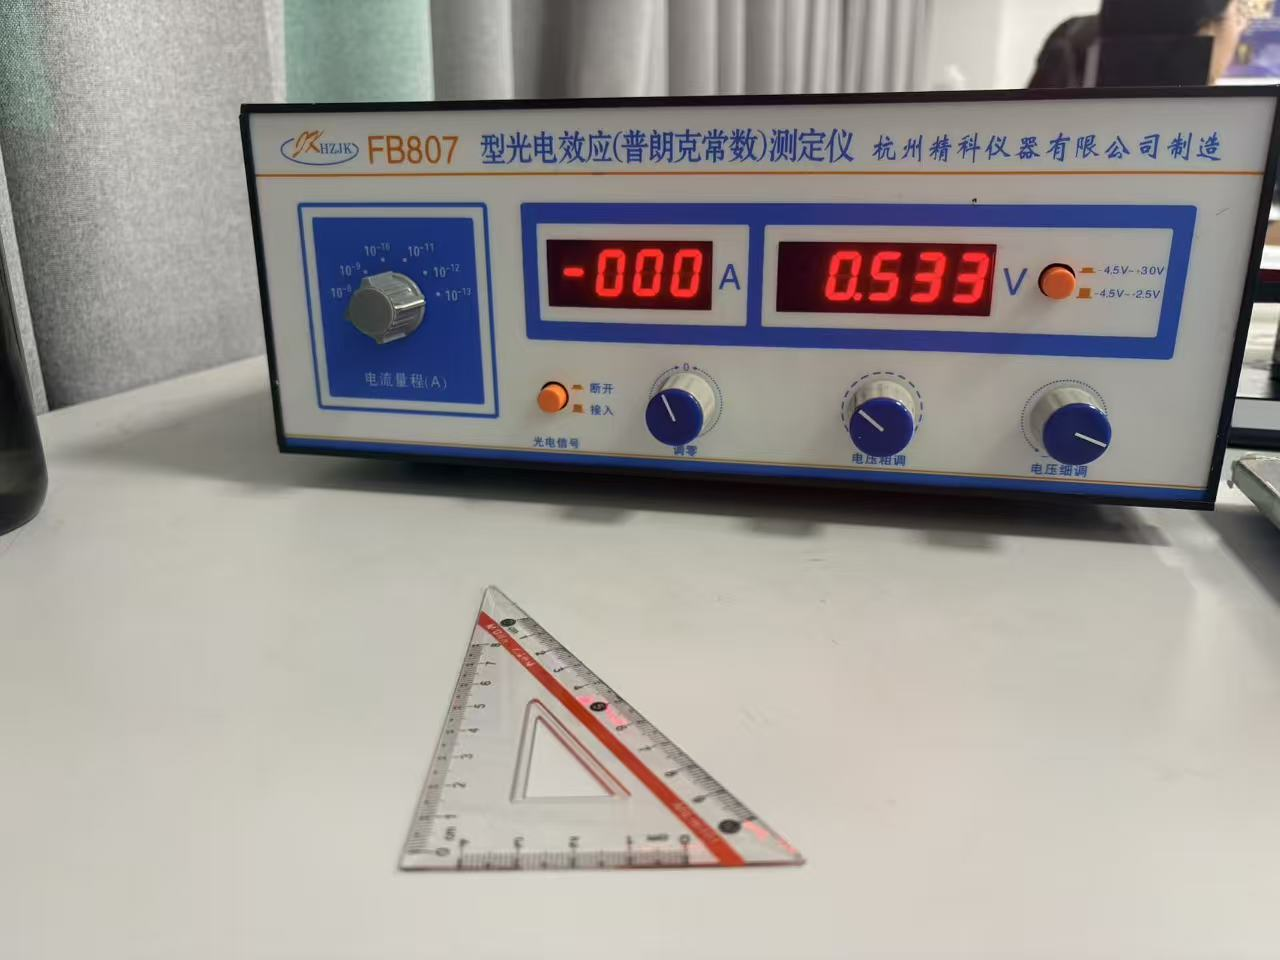
\includegraphics[height=3.5cm,width=0.98\linewidth,keepaspectratio]{../assets/debug-setup.jpg}
\caption{FB807 实验仪调试现场}
\end{figure}

原始测量记录如下。

\begin{figure}[H]\centering
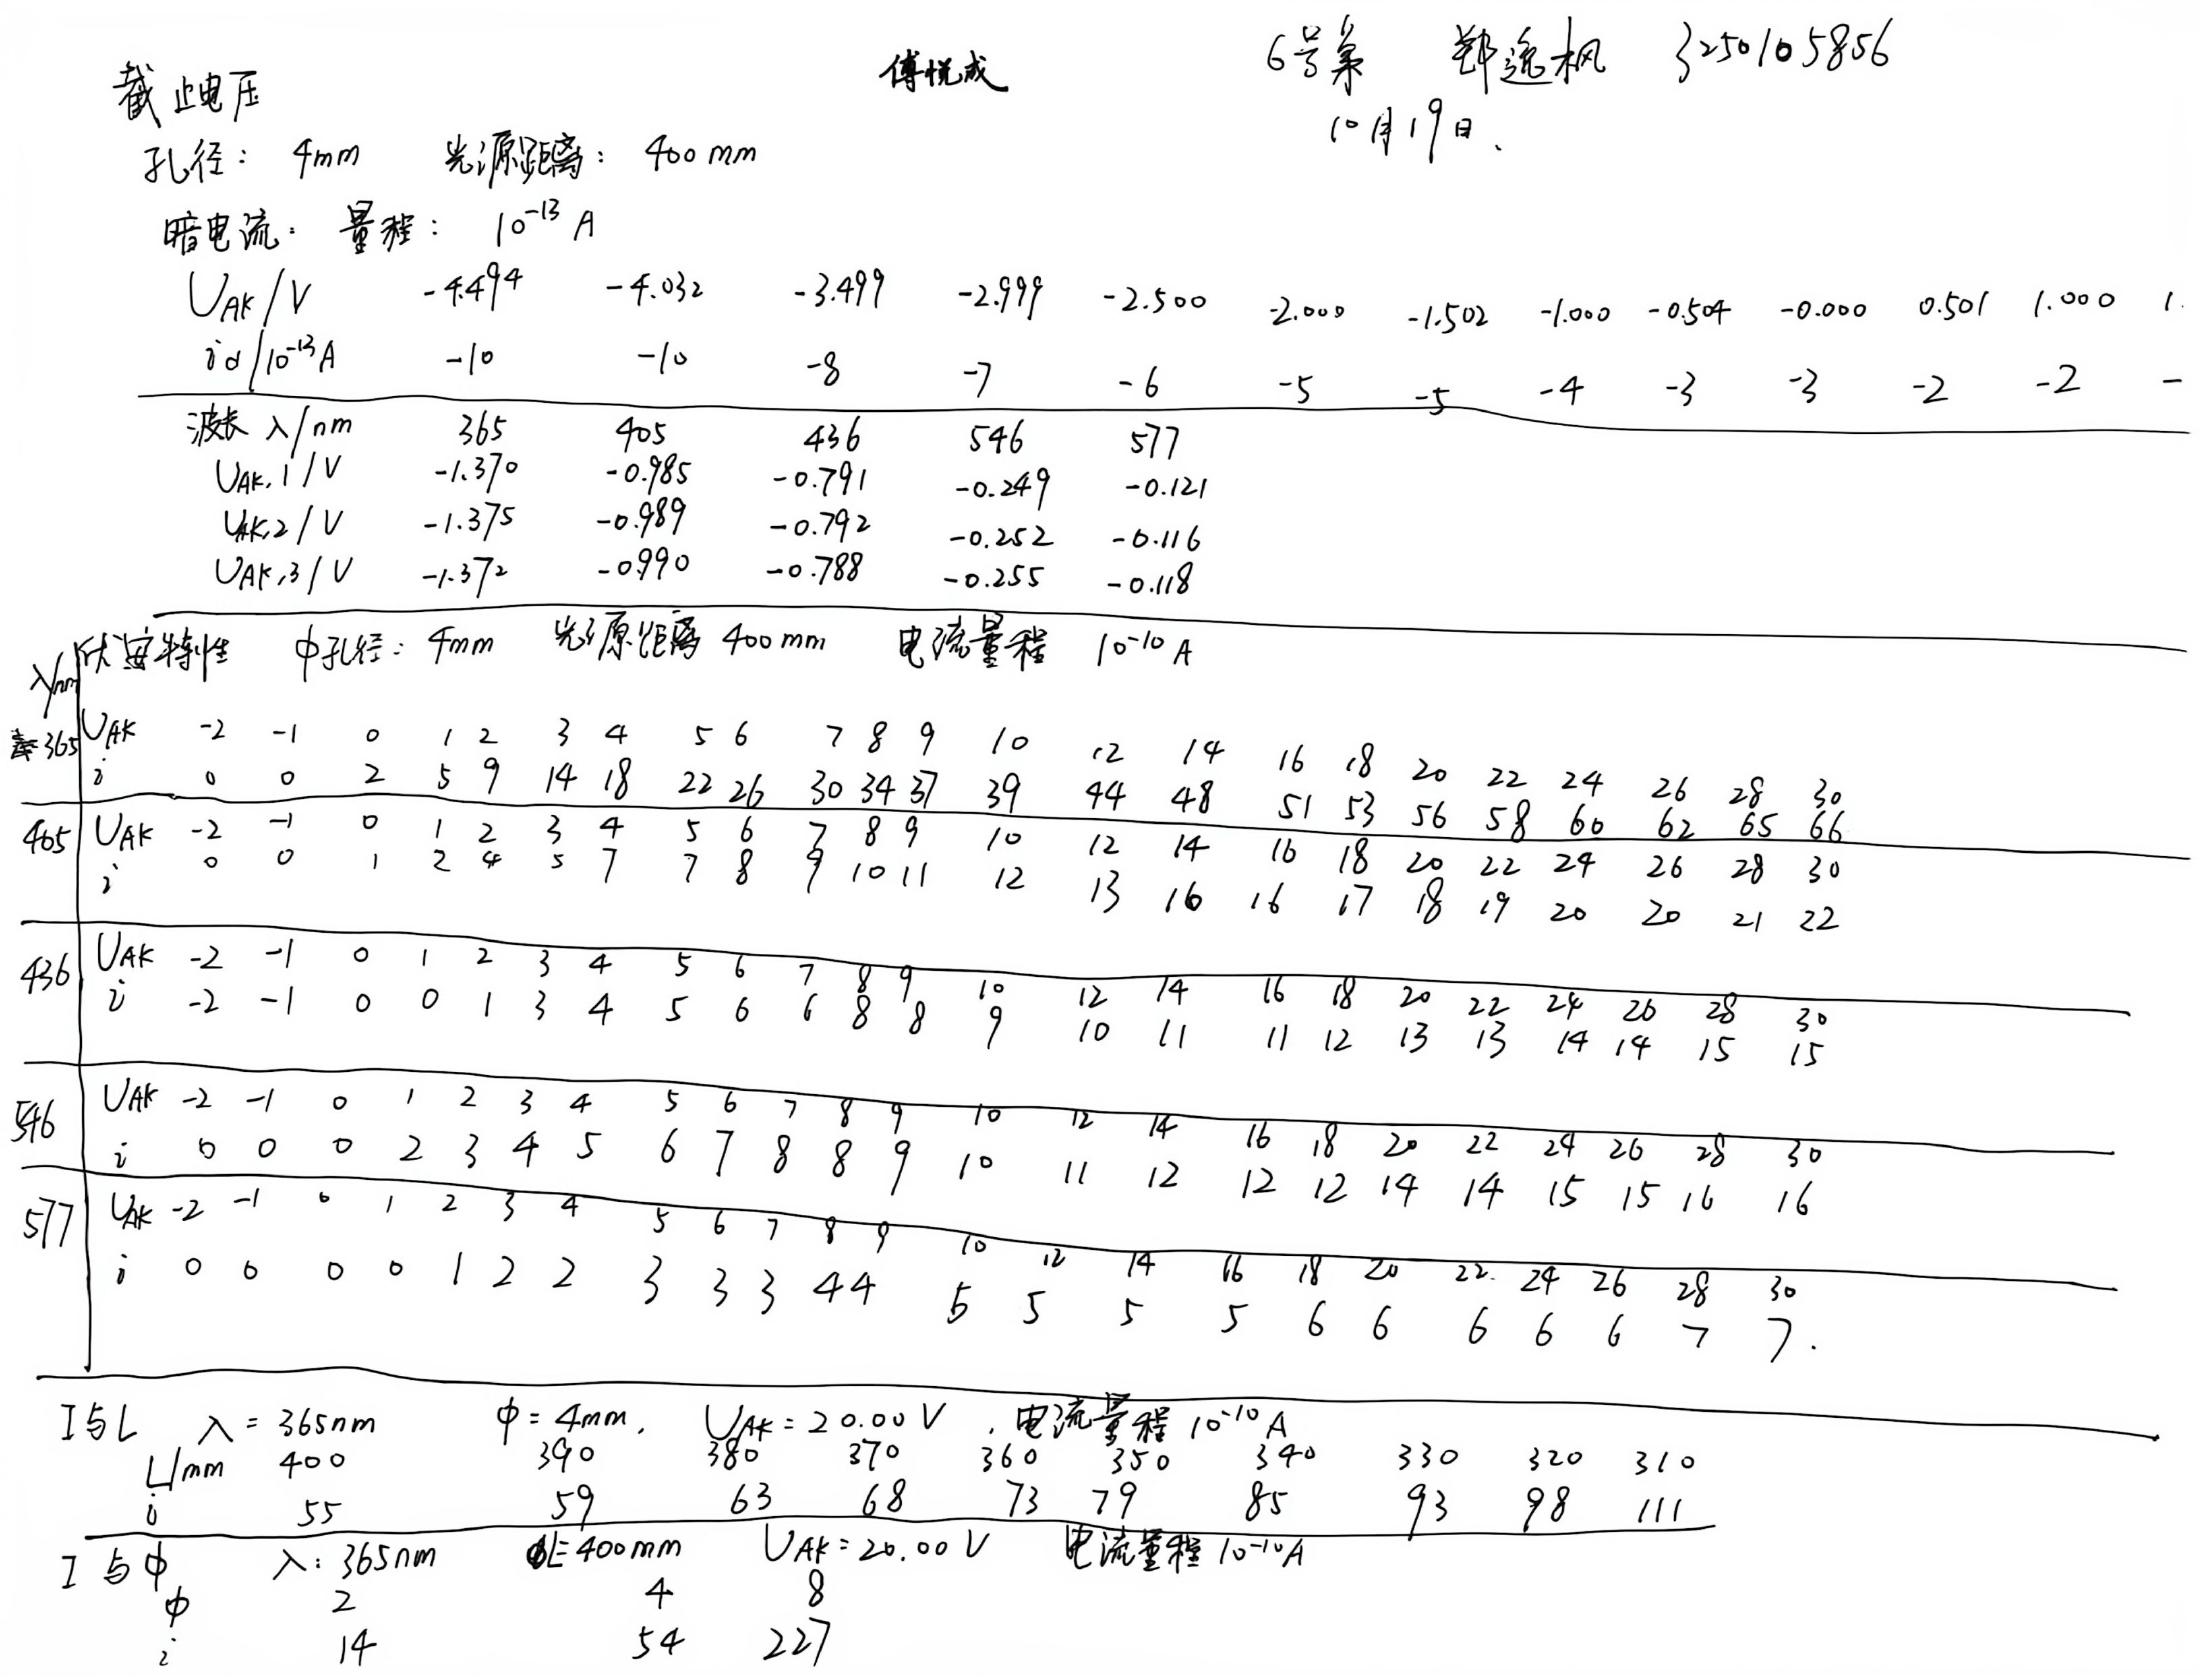
\includegraphics[height=9.5cm,width=0.98\linewidth,keepaspectratio]{../assets/raw-data.png}
\caption{本次原始测量记录（按阅读方向旋转）}
\end{figure}


\newpage
\subsection*{2. 截止电压与暗电流}

\begin{center}\small\setstretch{1.0}
\renewcommand{\arraystretch}{1.25}
\begin{tabular}{|c|c|c|c|}
\hline
$\lambda$/nm & $U_{AK,1}$/V & $U_{AK,2}$/V & $U_{AK,3}$/V\\\hline
365 & -1.370 & -1.375 & -1.372\\\hline
405 & -0.985 & -0.989 & -0.990\\\hline
436 & -0.791 & -0.792 & -0.788\\\hline
546 & -0.249 & -0.252 & -0.255\\\hline
577 & -0.121 & -0.116 & -0.118\\\hline
\end{tabular}
\end{center}

暗电流使用 $10^{-13}\,\mathrm A$ 档，伏安特性及两项拓展实验使用 $10^{-10}\,\mathrm A$ 档。

\begin{center}\small\setstretch{1.0}
\renewcommand{\arraystretch}{1.25}
\begin{tabular}{|c|c|}
\hline
$U_{AK}$/V & $i_d/(10^{-13}\,\mathrm A)$\\\hline
-0.000 & -3\\\hline
\end{tabular}
\end{center}



\subsection*{3. 拓展实验数据}

距离实验：$\lambda=365\,\mathrm{nm}$，$\Phi=4\,\mathrm{mm}$，$U_{AK}=20.00\,\mathrm V$。

\begin{center}\small\setstretch{1.0}
\renewcommand{\arraystretch}{1.25}
\begin{tabular}{|c|c|c|c|}
\hline
$L$/mm & $i/(10^{-10}\,\mathrm A)$ & $L$/mm & $i/(10^{-10}\,\mathrm A)$\\\hline
400 & 55 & 350 & 79\\\hline
390 & 59 & 340 & 85\\\hline
380 & 63 & 330 & 93\\\hline
370 & 68 & 320 & 98\\\hline
360 & 73 & 310 & 111\\\hline
\end{tabular}
\end{center}

孔径实验：$\lambda=365\,\mathrm{nm}$，$L=400\,\mathrm{mm}$，$U_{AK}=20.00\,\mathrm V$。

\begin{center}\small\setstretch{1.0}
\renewcommand{\arraystretch}{1.25}
\begin{tabular}{|c|c|c|c|}
\hline
$\Phi$/mm & 2 & 4 & 8\\\hline
$i/(10^{-10}\,\mathrm A)$ & 14 & 54 & 227\\\hline
\end{tabular}
\end{center}


\newpage
\subsection*{4. 完整伏安特性数据}

下表电流单位均为 $10^{-10}\,\mathrm A$。

\begin{center}\small\setstretch{1.0}
\renewcommand{\arraystretch}{1.25}
\begin{tabular}{|c|c|c|c|c|c|}
\hline
$U_{AK}$/V & 365 nm & 405 nm & 436 nm & 546 nm & 577 nm\\\hline
-2 & 0 & 0 & -2 & 0 & 0\\\hline
-1 & 0 & 0 & -1 & 0 & 0\\\hline
0 & 2 & 1 & 0 & 0 & 0\\\hline
1 & 5 & 2 & 0 & 2 & 0\\\hline
2 & 9 & 4 & 1 & 3 & 1\\\hline
3 & 14 & 5 & 3 & 4 & 2\\\hline
4 & 18 & 7 & 4 & 5 & 2\\\hline
5 & 22 & 7 & 5 & 6 & 3\\\hline
6 & 26 & 8 & 6 & 7 & 3\\\hline
7 & 30 & 9 & 6 & 8 & 3\\\hline
8 & 34 & 10 & 8 & 8 & 4\\\hline
9 & 37 & 11 & 8 & 9 & 4\\\hline
10 & 39 & 12 & 9 & 10 & 5\\\hline
12 & 44 & 13 & 10 & 11 & 5\\\hline
14 & 48 & 16 & 11 & 12 & 5\\\hline
16 & 51 & 16 & 11 & 12 & 5\\\hline
18 & 53 & 17 & 12 & 12 & 6\\\hline
20 & 56 & 18 & 13 & 14 & 6\\\hline
22 & 58 & 19 & 13 & 14 & 6\\\hline
24 & 60 & 20 & 14 & 15 & 6\\\hline
26 & 62 & 20 & 14 & 15 & 6\\\hline
28 & 65 & 21 & 15 & 16 & 7\\\hline
30 & 66 & 22 & 15 & 16 & 7\\\hline
\end{tabular}
\end{center}


